\chapter{Large Language Models}
\label{chap:llm}

A large language model computes a probability distribution over the next unit of text, given the text read so far, and an output is obtained by selecting from that distribution. This chapter reviews how that computation is defined, the Transformer architecture that carries it out, and the properties that emerge as the architecture is scaled to its current size. The chapter also introduces the hidden states, the internal representations that a single call to the model produces alongside its output. It also reviews how the truthfulness of a statement or the tool a model is about to call can be linearly decoded from these states.

\section{Language Modeling}
\label{sec:language-modeling}

\subsection{The next-token prediction task}
\label{subsec:next-token}

A language model assigns a probability to a piece of text. The model does not read whole words, but tokens, smaller pieces of text into which words are segmented; Section~\ref{sec:transformer} defines tokenization precisely. The formulation used by every model discussed in this work is predictive: given the part of the text that has already been read, the model assigns a probability to each token that can come next \cite[Chap.~24]{russellArtificialIntelligenceModern2022}, \cite{zhaoSurveyLargeLanguage2026}. Let $x_1, \dots, x_{i-1}$ denote the tokens already read. The model computes the probability of each token it knows being the next one:

\begin{equation}
    P(x_i \mid x_1, \dots, x_{i-1}).
\end{equation}

The probability of a complete text of $n$ tokens factorizes into the product of these probabilities:

\begin{equation}
    \label{eq:factorization}
    P(x_1, \dots, x_n) = \prod_{i=1}^{n} P(x_i \mid x_1, \dots, x_{i-1}).
\end{equation}

This factorization is what makes text generation a repeated application of the same prediction \cite[Chap.~24]{russellArtificialIntelligenceModern2022}. The task is long-standing, and the formulation has outlasted several generations of the models that implement it \cite{zhaoSurveyLargeLanguage2026}.

This predictive formulation has two consequences for how the model is used. It produces a distribution and not an answer, so an answer is obtained only by selecting from that distribution. It also reads only the text supplied to it, so everything that has to influence the prediction has to be part of that text. Both properties hold regardless of how the model is built.

\subsection{From counting to learned functions}
\label{subsec:counting-to-learned}

The conditional probability in Equation~\ref{eq:factorization} can be estimated from a corpus in more than one way. The earliest estimate is a statistical one: n-gram models count occurrences in the corpus and base each prediction on a fixed number of preceding tokens, regardless of how much text precedes them \cite{zhaoSurveyLargeLanguage2026}, \cite[Chap.~24]{russellArtificialIntelligenceModern2022}.

Neural language models replace the counting estimate with a learned function. A recurrent network reads the text one token at a time. To process token $x_i$, it combines that token with the representation produced after token $x_{i-1}$, and produces a new representation as output. This new representation carries information from every earlier token, so the prediction is no longer limited to the fixed number of preceding tokens that an n-gram model uses \cite{zhaoSurveyLargeLanguage2026}, \cite[Chap.~25]{russellArtificialIntelligenceModern2022}. This sequential dependency constrains training: the representation for token $x_i$ cannot be computed before the representation for token $x_{i-1}$ exists, so tokens cannot be processed in parallel, and information relating two distant tokens must pass through every intermediate representation \cite[Chap.~25]{russellArtificialIntelligenceModern2022}, \cite{vaswaniAttentionAllYou2023}.

Vaswani et al. proposed the Transformer, an architecture that removes this sequential dependency. The Transformer relies on attention, a mechanism that connects any two token positions directly, without passing information through the positions between them \cite{vaswaniAttentionAllYou2023}. Because a token's representation no longer depends on the representation of the token before it, every position can be processed in parallel. The Transformer was adopted in place of recurrent networks and underlies all subsequent large language models \cite{zhaoSurveyLargeLanguage2026}. Large pretrained Transformer language models are what the term Large Language Model refers to \cite{zhaoSurveyLargeLanguage2026}, and the rest of this chapter is concerned with them.

\section{The Transformer Architecture}
\label{sec:transformer}

The architecture Vaswani et al. proposed is composed of two parts \cite{vaswaniAttentionAllYou2023}, \cite[Chap.~25]{russellArtificialIntelligenceModern2022}:
\begin{itemize}
    \item the \emph{encoder} maps the input sequence to a sequence of internal representations;
    \item the \emph{decoder} produces an output sequence, predicting each token from the encoder output and from the tokens already generated.
\end{itemize}

Current generative language models are decoder-only, comprising the decoder part alone, which predicts the next token from the preceding ones without a separate encoder \cite[Chap.~25]{russellArtificialIntelligenceModern2022}. With no encoder to hold a separate input sequence, the query and the tokens generated so far occupy positions of the same single sequence. Generation is autoregressive: each emitted token is appended to that sequence before the next one is predicted \cite{zhaoSurveyLargeLanguage2026}. The number of preceding tokens a prediction can use is fixed and is defined as the context window \cite{zhaoSurveyLargeLanguage2026}. The models used in this work are of this kind, and the remainder of this section describes one call to a decoder-only model, one step at a time: the query is segmented into tokens, the tokens are converted into vectors, a stack of identical blocks transforms these vectors into a new vector per token position, and the vector at the last position is converted into the distribution from which the emitted token is selected.

\subsection{Tokens}
\label{subsec:tokens}

\emph{Tokens} are the units of a fixed vocabulary into which text is segmented before it is processed \cite{zhaoSurveyLargeLanguage2026}. Tokenization is performed by subword methods, which keep frequent words as single units and split rarer ones into smaller pieces, so that any input can be represented with a vocabulary of bounded size \cite{zhaoSurveyLargeLanguage2026}, \cite[Chap.~24]{russellArtificialIntelligenceModern2022}. A token is therefore not a linguistic unit, and one word can correspond to several tokens. Everything the model reads and everything it emits is a sequence of tokens, and the positions referred to throughout this chapter are token positions.

As an example, Table~\ref{tab:tokenization-example} shows how a byte-pair-encoding tokenizer segments the word \texttt{unbelievability} into four tokens. The boundaries do not follow the parts of the word that carry meaning: \emph{unbelievability} is split with \texttt{v} separated from \texttt{belie} rather than kept together as \texttt{believ}.

\begin{table}[ht]
    \centering
    \renewcommand{\arraystretch}{1.2}
    \begin{tabular}{@{}ll@{}}
        \toprule
        Token ID & Token text \\
        \midrule
        359 & \texttt{un} \\
        32898 & \texttt{belie} \\
        85 & \texttt{v} \\
        2968 & \texttt{ability} \\
        \bottomrule
    \end{tabular}
    \caption[Tokenization of \texttt{unbelievability} by a byte-pair-encoding tokenizer]{Tokenization of \texttt{unbelievability} by a byte-pair-encoding tokenizer.}
    \label{tab:tokenization-example}
\end{table}

\subsection{Embedding: tokens to vectors}
\label{subsec:embedding}

Each token of the vocabulary is associated with a learned vector of dimension $d_{\mathrm{model}}$. The input sequence is converted into the corresponding sequence of vectors before it reaches the first block \cite{vaswaniAttentionAllYou2023}. Attention, defined in Section~\ref{subsec:attention}, relates any two positions with the same operation regardless of where they occur in the sequence, so it carries no notion of order on its own. Information about the position of each token is therefore supplied separately and combined with the token vector, so that two identical tokens at different positions do not enter the stack with the same representation \cite{vaswaniAttentionAllYou2023}. This added information is called the \emph{positional encoding} \cite{vaswaniAttentionAllYou2023}. The result is one vector per token position, which is the input of the first block.

Table~\ref{tab:positional-encoding-example} shows this combination for the four tokens of \texttt{unbelievability} from Table~\ref{tab:tokenization-example}.

\begin{table}[H]
  \centering
  \renewcommand{\arraystretch}{1.2}
  \begin{tabular}{@{}lccc@{}}
    \toprule
    Token & Token embedding & Positional encoding & Input vector \\
    \midrule
    \texttt{un}      & $e_{\mathtt{un}}$      & $p_1$ & $e_{\mathtt{un}} + p_1$ \\
    \texttt{belie}   & $e_{\mathtt{belie}}$   & $p_2$ & $e_{\mathtt{belie}} + p_2$ \\
    \texttt{v}       & $e_{\mathtt{v}}$       & $p_3$ & $e_{\mathtt{v}} + p_3$ \\
    \texttt{ability} & $e_{\mathtt{ability}}$ & $p_4$ & $e_{\mathtt{ability}} + p_4$ \\
    \bottomrule
  \end{tabular}
  \caption[Positional encoding example for \texttt{unbelievability}]{Positional encoding example for \texttt{unbelievability}.}
  \label{tab:positional-encoding-example}
\end{table}

\subsection{Attention}
\label{subsec:attention}

Attention is a mechanism that computes, for each pair of tokens, a weight reflecting their relevance to each other \cite{vaswaniAttentionAllYou2023}, \cite[Chap.~25]{russellArtificialIntelligenceModern2022}. Each token is then represented as a sum of the representations of every other token, weighted by these values. This sum includes a distant token's representation in the same step as a neighboring one's, unlike the recurrent computation of Section~\ref{subsec:counting-to-learned}, where information about a distant token has to pass through the representation of every token between it and the current position \cite{vaswaniAttentionAllYou2023}.

The mechanism operates on three sets of vectors derived from the token representations, the queries, keys, and values \cite{vaswaniAttentionAllYou2023}. With these arranged into matrices $Q$, $K$, and $V$, scaled dot-product Attention is computed as
\begin{equation}
    \mathrm{Attention}(Q, K, V) = \mathrm{softmax}\!\left(\frac{QK^\top}{\sqrt{d_k}}\right) V ,
\end{equation}
where $d_k$ is the dimension of the queries and keys \cite{vaswaniAttentionAllYou2023}. Each operation in the expression has a distinct role:
\begin{itemize}
    \item the product $QK^\top$ scores each query against every key through their dot product;
    \item the division by $\sqrt{d_k}$ prevents the scores from growing too large, which would push the softmax into a region where its gradients are too small for training to proceed \cite{vaswaniAttentionAllYou2023};
    \item the softmax normalizes the scores into weights that sum to one, so that each output is the corresponding weighted sum of the values \cite{vaswaniAttentionAllYou2023}.
\end{itemize}
In the Transformer architecture, this computation is carried out in parallel by several Attention heads, each operating over a distinct learned subspace, so that different relations between tokens can be represented simultaneously \cite{vaswaniAttentionAllYou2023}. $Q$, $K$, and $V$ are each projected by a separate learned matrix per head, $h$ instances of scaled dot-product Attention are computed independently, one per head, and the resulting vectors are concatenated and projected once more:
\begin{equation}
    \mathrm{MultiHead}(Q, K, V) = \mathrm{Concat}(\mathrm{head}_1, \ldots, \mathrm{head}_h) W^O, \quad \mathrm{head}_i = \mathrm{Attention}(Q W_i^Q, K W_i^K, V W_i^V),
\end{equation}
where $W_i^Q$, $W_i^K$, $W_i^V$, and $W^O$ are learned projection matrices \cite{vaswaniAttentionAllYou2023}. Vaswani et al. motivate this design as follows. A single Attention head averages over all relations between two positions into one weighted sum, and cannot represent them separately. Multiple heads let the model attend to information from different representation subspaces at once \cite{vaswaniAttentionAllYou2023}.

During training, the whole sequence is processed at once, for efficiency. Without a constraint, the weighted sum at a position could include the very token it is meant to predict, and the model would learn to copy it instead of predicting it from context. Vaswani et al. introduced masking in the decoder to prevent this: the weighted sum at position $i$ is restricted to the first $i$ tokens, so the representation at that position reflects only what precedes it \cite{vaswaniAttentionAllYou2023}. This keeps training consistent with generation, where the tokens after position $i$ do not yet exist when it is predicted.

This parallelism, already noted in Section~\ref{sec:language-modeling} for the architecture as a whole, and the capacity it enables made it possible to scale language models to hundreds of billions of parameters \cite{zhaoSurveyLargeLanguage2026}.

\subsection{The block}
\label{subsec:block}

A decoder-only Transformer is a stack of $L$ identical blocks. The blocks are applied in sequence: the output of one block is the input to the next. Each block has two sublayers: multi-head Attention, the only component that moves information between positions, and a position-wise feed-forward sublayer, applied to each position separately \cite{vaswaniAttentionAllYou2023}. Vaswani et al. call this two-sublayer block the encoder layer, and build the decoder layer by adding a third sublayer that attends to the encoder output \cite{vaswaniAttentionAllYou2023}. A decoder-only model stacks copies of the encoder layer alone, since it has no separate encoder.

Each sublayer is wrapped in a residual connection followed by layer normalization, so that the output of a sublayer is added to its input rather than replacing it \cite{vaswaniAttentionAllYou2023}. The vector carried from one block to the next at a given position is therefore the sum of the input embedding and the contributions written by every sublayer below it.

\subsection{Dense and mixture-of-experts blocks}
\label{subsec:dense-moe}

In the architecture described so far, the feed-forward sublayer of a block is a single module applied to every token, so all of its parameters take part in the computation of every position. A model whose blocks are built in this way is called dense: its total parameter count and the compute required per token grow together \cite{zhangMixtureExpertsLarge2025}. This coupling bounds how far the parameter count can be increased at a fixed training and inference cost, and the mixture-of-experts architecture is the variant that decouples the two \cite{zhangMixtureExpertsLarge2025}.

A mixture-of-experts layer replaces the single feed-forward sublayer with a set of $N$ parallel sublayers, called \emph{experts}, together with a gating function that selects a sparse subset of them for each input \cite{zhangMixtureExpertsLarge2025}. The experts are typically independent feed-forward modules \cite{zhangMixtureExpertsLarge2025}. The output of the mixture-of-experts layer is the weighted combination
\begin{equation}
    y = \sum_{i=1}^{N} g_i(x) E_i(x) ,
\end{equation}
where $E_i(x)$ is the output of expert $i$ and $g_i(x)$ is the gating function, which assigns a nonzero weight to at most $k \ll N$ experts \cite{zhangMixtureExpertsLarge2025}. The gating function is commonly implemented by top-$k$ routing, which scores each expert against the input and masks all but the $k$ largest scores before the weights are normalized \cite{zhangMixtureExpertsLarge2025}.

Because only $k$ experts are evaluated, the computational cost of the layer depends on the number of selected experts and not on the size of the expert pool \cite{zhangMixtureExpertsLarge2025}. The total number of parameters of the model and the number of parameters used for one token are therefore distinct quantities. This separation allows models with hundreds of billions of parameters to be trained and served at a compute cost far below that of a dense model of the same size \cite{zhangMixtureExpertsLarge2025}. Switch Transformer and GLaM activate one or two experts per token out of 64 \cite{zhangMixtureExpertsLarge2025}. The selection is made per token and per layer, so different tokens of the same sequence are processed by different experts.

Training a mixture-of-experts layer is subject to expert collapse, where a few experts receive most inputs and the rest remain underused; an auxiliary load-balancing objective is added to the training loss to counter it, at the cost of some expert specialization \cite{zhangMixtureExpertsLarge2025}. At inference, sparse activation produces irregular memory access and cross-device communication, which raises latency \cite{zhangMixtureExpertsLarge2025}.

Both kinds of block are present in the current open-weight families, in proportions that vary from one family to another. For instance, the Qwen3 and Gemma 4 series contain dense models and mixture-of-experts models \cite{yangQwen3TechnicalReport2025, teamGemma4Technical2026}, gpt-oss-120b and gpt-oss-20b are mixture-of-experts models \cite{openaiGptoss120bGptoss20bModel2025}, and the largest model of the Llama 3 series is a dense Transformer of 405B parameters \cite{grattafioriLlama3Herd2024}. The dense/mixture-of-experts choice affects only the feed-forward sublayer of each block. The sequence of blocks, the residual connections, and the vector carried at each position are identical between the two kinds, so every property described in the rest of this chapter holds for both.

\subsection{The residual stream through the block stack}
\label{subsec:residual-stream}

Because each sublayer adds its output to its input rather than replacing it (Section~\ref{subsec:block}), the vector at a given position is not replaced by each block but extended by it. The quantity carried through the block stack at one position is therefore an accumulating representation, read and written by every block in turn. This accumulating representation is what the term \emph{residual stream} refers to.

Geva et al. analyzed the feed-forward sublayers under this reading and reported that their output is refined throughout the layers of the model via the residual connections, with lower layers capturing shallow patterns and upper layers more semantic ones \cite{gevaTransformerFeedForwardLayers2021}. Belrose et al. described the resulting computation as iterative inference, in which the prediction is refined block by block \cite{belroseElicitingLatentPredictions2025}. Both analyses treat the vector carried across the block stack as an accumulating representation that later blocks read and write.

\subsection{The unembedding and the output distribution}
\label{subsec:unembedding}

The block stack produces one vector per position, and the distribution over the next token is computed from the vector at the last position alone. That vector is mapped to one score per vocabulary entry by a linear transformation, and the scores are normalized into a probability distribution by a softmax function \cite{vaswaniAttentionAllYou2023}. The linear transformation is referred to as the unembedding, and it is the inverse counterpart of the embedding of Section~\ref{subsec:embedding}, mapping from the model's representation space back to the vocabulary. The output of the model is therefore a linear readout of a single vector, followed by a normalization.

\subsection{Decoding: from distribution to token}
\label{subsec:decoding}

The distribution over the vocabulary is not itself an output token. A decoding strategy selects one token from it. The same trained model can be run with different decoding strategies, since the choice is made when generating text, not fixed during training \cite{zhaoSurveyLargeLanguage2026}. Under \emph{greedy decoding} the token with the highest probability is selected at each step \cite{zhaoSurveyLargeLanguage2026}, so the selection rule itself introduces no randomness. Under sampling the token is drawn from the distribution, which is commonly modified before the draw by two operations that act at different points:
\begin{itemize}
    \item \emph{temperature scaling} rescales the distribution, dividing the scores by a constant before the softmax, so that values below one concentrate it on the most probable tokens and values above one flatten it \cite{zhaoSurveyLargeLanguage2026};
    \item \emph{top-p sampling}, also called nucleus sampling, truncates the distribution, restricting the draw to the smallest set of tokens whose cumulative probability exceeds a threshold $p$ \cite{zhaoSurveyLargeLanguage2026}.
\end{itemize}
Neither operation selects a token on its own, and both leave the emitted token random. Two runs on the same input can therefore return different sequences, but under greedy decoding they cannot. Section~\ref{sec:properties} states the consequences of this for systems built on the model.

\subsection{Generating a sequence: prefill and decode}
\label{subsec:prefill-decode}

The steps above produce one token, and the model is queried again on the sequence extended by it \cite{zhaoSurveyLargeLanguage2026}, until the sequence terminates. The computation therefore separates into two phases. In the first phase, the input supplied by the caller is processed in a single forward pass, which is possible because Attention introduces no sequential dependency between positions and all its positions are computed in parallel \cite{vaswaniAttentionAllYou2023}. In the second phase, tokens are produced one at a time, one forward pass per token \cite{zhaoSurveyLargeLanguage2026}. The two phases are commonly referred to as \emph{prefill} and \emph{decode}.

\begin{figure}[ht]
	\centering
	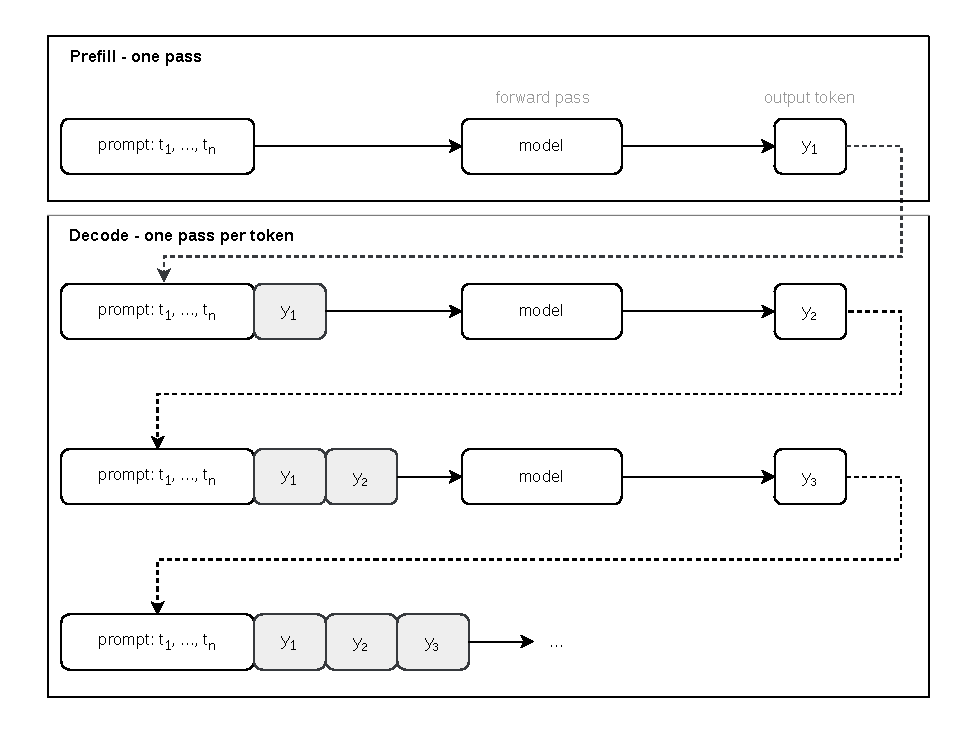
\includegraphics[width=0.9\textwidth]{images/prefill_decode.pdf}
	\caption[Prefill and decode]{Prefill and decode. Prefill processes the whole prompt in a single forward pass and emits the first token. Decode performs one forward pass per token, each time on the input extended by the token emitted at the previous step.}
	\label{fig:prefill-decode}
\end{figure}

The keys and values computed during prefill and at each decode step are stored in the key-value cache \cite{xuKVCacheOptimization2026}. Each decode step then computes attention only for the new token, using the cached keys and values, instead of recomputing attention for all previous tokens.

The distinction between prefill and decode matters for cost. The vectors produced at the last prompt token are produced by the prefill pass, which is executed in any case before the first output token can be emitted. Obtaining them therefore requires no additional forward pass, and no generated tokens. A method that reads the prefill representation and a method that reads the generated text differ in when they can act: the first can act before decoding begins, the second only after it has finished.

\section{Scale, Emergence, and Adaptation}
\label{sec:scale-emergence}

The mechanism described in Section~\ref{sec:transformer} is the same at every model size. Scale changes the range of tasks the model can be used for, instruction tuning changes the form in which a task is supplied to it, and the interface exposed by the provider changes the form in which the answer is returned.

\subsection{Scale and emergent abilities}
\label{subsec:scale}

Transformer-based language models have been scaled to progressively larger sizes. Once pretrained models reached on the order of a hundred billion parameters, their behavior diverged from that of smaller predecessors. In 2020, Brown et al. reported that GPT-3 could perform a wide range of tasks given only a natural-language prompt and a few examples, with no gradient updates \cite{brownLanguageModelsAre2020}. A separate line of work has identified \emph{emergent abilities}, capabilities such as multi-step reasoning and multi-digit arithmetic that do not improve smoothly with scale but appear only beyond a certain model size \cite{weiEmergentAbilitiesLarge2022, zhaoSurveyLargeLanguage2026}.

\subsection{Foundation models and adaptation by prompt}
\label{subsec:foundation-models}

A Large Language Model (or LLM) is an instance of a foundation model: a model trained on broad data, generally through self-supervision at scale, that can be adapted to a wide range of downstream tasks rather than trained for any one of them \cite{bommasaniOpportunitiesRisksFoundation2022}. Bommasani et al. chose the term \emph{foundation} to name this role: the model is itself incomplete, but it serves as the common basis from which many task-specific models are built through adaptation \cite{bommasaniOpportunitiesRisksFoundation2022}. The breadth of the training data reduces the need to encode task-specific information in the model, so one general model can replace many task-specific ones. The model can be adapted to a particular task by supplying a prompt that states the task in natural language, with no retraining \cite{bommasaniOpportunitiesRisksFoundation2022,brownLanguageModelsAre2020}. The task is therefore part of the input, and it occupies token positions of the sequence described in Section~\ref{sec:transformer} like any other content.

\subsection{Frozen models}
\label{subsec:frozen}

Adaptation by prompt changes no parameter of the model: the weights set during pretraining, and during any later fine-tuning, stay fixed while the model is used \cite{bommasaniOpportunitiesRisksFoundation2022,brownLanguageModelsAre2020}. A model whose parameters receive no gradient update while it is used, whether it is adapted by prompt or simply run as is, is referred to throughout this work as \emph{frozen}.

\subsection{Instruction tuning and the chat format}
\label{subsec:instruction-tuning}

Instruction following is not a direct result of scale: next-token prediction does not align the output with what a user intends, and larger models can be as untruthful or unhelpful as smaller ones \cite{ouyangTrainingLanguageModels2022}. Instruction tuning addresses this: a pretrained model is fine-tuned on demonstrations of desired behavior and then refined with reinforcement learning from human feedback, producing a system that follows natural-language instructions across many tasks \cite{ouyangTrainingLanguageModels2022, zhaoSurveyLargeLanguage2026}.

Instruction tuning also sets a fixed input format. Instruction-tuned models are queried through a chat format that delineates roles, such as a system instruction, a user message, and previous assistant turns \cite{openaiGptoss120bGptoss20bModel2025}. The prompt processed at inference time is the rendering of these roles into a single token sequence, as Section~\ref{sec:terminology} defines in detail.

\subsection{Chain-of-thought prompting}
\label{subsec:chain-of-thought}

Adaptation by prompt also covers how the answer is produced, and not only what task is asked. Wei et al. introduced \emph{chain-of-thought} prompting, in which the prompt contains demonstrations that state a series of intermediate reasoning steps before the answer. The model then generates the same kind of steps before its answer to the query \cite{weiChainofThoughtPromptingElicits2023}. They reported that the technique improves performance on arithmetic, commonsense, and symbolic reasoning tasks, and that prompting a 540B-parameter model with eight such demonstrations reaches state-of-the-art accuracy on the GSM8K benchmark of math word problems \cite{weiChainofThoughtPromptingElicits2023}. The gains appear only in sufficiently large models, which places the technique alongside the emergent abilities of Section~\ref{subsec:scale} \cite{weiChainofThoughtPromptingElicits2023, weiEmergentAbilitiesLarge2022}.

The intermediate steps are produced by ordinary token generation: each step is a span of tokens, emitted one at a time in the decode phase of Section~\ref{subsec:prefill-decode}, and each token is appended to the input before the next is predicted. The technique changes the sequence the answer is computed from: it now contains the model's own intermediate output.

Current model families make this behavior part of the model rather than of the prompt. Some expose it as a mode selected at inference time within one model \cite{yangQwen3TechnicalReport2025, teamGemma4Technical2026}, and some are released to produce chain-of-thought output by default \cite{openaiGptoss120bGptoss20bModel2025}.

\subsection{Structured output and function calling}
\label{sec:structured-output}

A language model emits tokens, so any output with a defined shape has to be produced as text that conforms to that shape. OpenAI introduced function calling as an API feature, later also referred to as tool calling. It makes this a first-class feature of the model interface \cite{FunctionCallingOther2024}. A set of functions is declared with names, descriptions, and argument schemas, and the model returns a structured object that names one of the declared functions and supplies its arguments, instead of free-form text \cite{FunctionCallingOther2024}.

The declarations are part of the prompt: the names, descriptions, and schemas of the available functions are rendered into the token sequence the model processes.

The model does not execute the function it calls. The calling application runs the named function with the supplied arguments, and the result is sent back to the model as a new turn. The model then continues generation using that result, typically to produce a final response that incorporates it \cite{FunctionCallingOther2024}.

\section{Defining the Prompt}
\label{sec:terminology}

Section~\ref{subsec:instruction-tuning} introduces the \emph{prompt} as the rendering of chat-format roles into one token sequence, together with other information such as function call definitions. However, the term prompt is also commonly used to name the request submitted to a model. This work distinguishes between the two senses, since the rest of it does not use them interchangeably.

\subsection{Query, turn, system prompt, and prompt}
\label{subsec:query-prompt}

The terms \emph{query}, \emph{input}, or \emph{request} name the text a user submits to a large language model. The \emph{response} is the sequence of tokens the model generates after a given request. Together, a request and its response form one \emph{turn} of a conversation. The model may also be invoked with a \emph{system prompt}, an instruction that states the model's role and the behavior it must follow, and is placed before the user turns in the rendered sequence \cite{openaiGptoss120bGptoss20bModel2025}. Finally, function calling declarations like the ones described in Section~\ref{sec:structured-output} (also known as \emph{tool definitions}) can be part of the information supplied to the model. Altogether, this information forms a single prompt, the actual content submitted to the model.

\begin{table}[htbp]
\centering
\begin{tabularx}{\textwidth}{@{}>{\raggedright\arraybackslash}p{0.27\textwidth}X@{}}
\toprule
\textbf{Term} & \textbf{What it names} \\
\midrule
\emph{query}, \emph{input}, or \emph{request} & one message a user submits to obtain a response \\[4pt]
\emph{response} & the text the model generates in response to a request \\[4pt]
\emph{turn} & a request together with the response it receives \\[4pt]
\emph{system prompt} & an instruction that states the model's role and the behavior it must follow, supplied by the application rather than by the user, and placed before the user turns in the rendered sequence \cite{openaiGptoss120bGptoss20bModel2025} \\[4pt]
\emph{prompt} & the full token sequence a model reads: the system prompt and every turn of the conversation so far, rendered together, plus any declared functions when function calling is enabled (Section~\ref{sec:structured-output}) \\
\bottomrule
\end{tabularx}
\caption[Terms for a query and its surrounding prompt]{The terms this work uses for a query and for the prompt built around it.}
\label{tab:terminology}
\end{table}


\subsection{A rendered example}
\label{subsec:rendered-example}

The rendering of the prompt is defined by a separate chat template. Figure~\ref{fig:rendered-example} shows how Qwen3-4B-Instruct \cite{yangQwen3TechnicalReport2025} renders this template when the query ``Are you able to research online?'' is submitted to a model, together with a specific system prompt and a tool definition that allows the model to request a web search.

\begin{figure}[htbp]
\centering
\footnotesize
\begin{tabularx}{\textwidth}{X}
\toprule
\texttt{<|im\_start|>system} \\
\texttt{You are a helpful assistant. You can search online if you need current information.} \\
\texttt{\# Tools} \\
\texttt{You may call one or more functions to assist with the user query. You are} \\
\texttt{provided with function signatures within <tools></tools> XML tags:} \\
\texttt{<tools>} \\
\texttt{\{"type": "function", "function": \{"name": "web\_search", "description":} \\
\texttt{"Search the web for a query and return matching results.", "parameters":} \\
\texttt{\{"type": "object", "properties": \{"query": \{"type": "string", "description":} \\
\texttt{"The search query."\}\}, "required": ["query"]\}\}\}} \\
\texttt{</tools>} \\
\texttt{For each function call, return a json object with function name and arguments} \\
\texttt{within <tool\_call></tool\_call> XML tags:} \\
\texttt{<tool\_call>} \\
\texttt{\{"name": <function-name>, "arguments": <args-json-object>\}} \\
\texttt{</tool\_call><|im\_end|>} \\
\texttt{<|im\_start|>user} \\
\texttt{Are you able to research online?<|im\_end|>} \\
\texttt{<|im\_start|>assistant} \\
\bottomrule
\end{tabularx}
\caption[Full prompt rendered with the Qwen3-4B-Instruct chat template]{A full prompt rendered using the Qwen3-4B-Instruct chat template.}
\label{fig:rendered-example}
\end{figure}

The rendered sequence ends right after the \texttt{assistant} role tag, with no content after it. This is the point where generation starts, and it corresponds to the last prompt token discussed in Section~\ref{subsec:last-token}.

Each call to the model is stateless: nothing from a prior call is retained, so any content the model must read again is included in any subsequent prompt.

Suppose the model answers the request of Figure~\ref{fig:rendered-example} with ``Yes, I can search the web if the question needs current information.'', completing the first turn, and the user then asks ``What is the weather in London today?''. Figure~\ref{fig:rendered-example-2} shows the prompt for this second call. The system prompt and the tool declaration are unchanged from Figure~\ref{fig:rendered-example} and are rendered again in full. What is added is the first turn and the new request.

\begin{figure}[htbp]
\centering
\scriptsize
\begin{tabularx}{\textwidth}{X}
\toprule
\texttt{<|im\_start|>system} \\
\texttt{You are a helpful assistant. You can search online if you need current information.} \\
\texttt{\# Tools} \\
\texttt{You may call one or more functions to assist with the user query. You are} \\
\texttt{provided with function signatures within <tools></tools> XML tags:} \\
\texttt{<tools>} \\
\texttt{\{"type": "function", "function": \{"name": "web\_search", "description":} \\
\texttt{"Search the web for a query and return matching results.", "parameters":} \\
\texttt{\{"type": "object", "properties": \{"query": \{"type": "string", "description":} \\
\texttt{"The search query."\}\}, "required": ["query"]\}\}\}} \\
\texttt{</tools>} \\
\texttt{For each function call, return a json object with function name and arguments} \\
\texttt{within <tool\_call></tool\_call> XML tags:} \\
\texttt{<tool\_call>} \\
\texttt{\{"name": <function-name>, "arguments": <args-json-object>\}} \\
\texttt{</tool\_call><|im\_end|>} \\
\texttt{<|im\_start|>user} \\
\texttt{Are you able to research online?<|im\_end|>} \\
\texttt{<|im\_start|>assistant} \\
\texttt{Yes, I can search the web if the question needs current information.<|im\_end|>} \\
\texttt{<|im\_start|>user} \\
\texttt{What is the weather in London today?<|im\_end|>} \\
\texttt{<|im\_start|>assistant} \\
\bottomrule
\end{tabularx}
\caption[Next-call prompt rendered with Qwen3-4B-Instruct chat template]{The prompt for the next call in the same conversation, rendered using the Qwen3-4B-Instruct chat template.}
\label{fig:rendered-example-2}
\end{figure}

The whole conversation, not only the new request, is resent at every call. An LLM can therefore handle conversations despite being completely stateless.

\section{Constraints and Limitations}
\label{sec:properties}

The properties of large language models stated in this section constrain what any system built around them can guarantee. They are consequences of how the model is trained and queried, and they are stated here because the rest of this work depends on them.

\paragraph{Stochasticity.} Each output of a large language model is sampled from a distribution over tokens rather than read from a deterministic policy, according to the decoding strategy of Section~\ref{subsec:decoding}. Two runs on the same input can therefore return different outputs. Song et al. showed that this variability is large enough to affect benchmark conclusions \cite{songGoodBadGreedy2024}. The same model can score differently under greedy decoding and under sampling, and the gap is observed across model families and benchmarks \cite{songGoodBadGreedy2024}. The same analysis reported that the ranking of two models can change with the decoding configuration, so a comparison between models holds only for a fixed configuration \cite{songGoodBadGreedy2024}. The effect compounds in a system that chains many model calls: the variance of each call carries into the next, so two runs on the same task can reach different outcomes through different paths.

\paragraph{Context dependence.} Model behavior depends on the prompt and on whatever else occupies the context window, not on encoded rules or a stable policy. The position of the relevant content in the context is one factor. By keeping the input fixed and moving the document that contains the answer, Liu et al. reported that performance is highest when that document is at the beginning or at the end of the input context and degrades when the model must use it in the middle \cite{liuLostMiddleHow2023a}. The performance of GPT-3.5-Turbo on multi-document question answering drops by more than 20\% under this change, and when the answer document is placed in the middle of the context (the worst position), performance is lower than that of the same model with no documents supplied at all \cite{liuLostMiddleHow2023a}. Models with an extended context window are not better at using their input context than their non-extended counterparts \cite{liuLostMiddleHow2023a}. The effective policy is implicit in the model and in the context assembled around it, and it shifts whenever any part of that context changes.

\paragraph{Instruction following.} Instructions in the prompt state what the model is asked to do, and those instructions are not always followed. Zhou et al. measured this on instructions whose satisfaction a program can check, such as a word limit or a required keyword, using 25 instruction types over about 500 prompts \cite{zhouInstructionFollowingEvaluationLarge2023}. GPT-4 satisfies every verifiable instruction of a prompt in 76.89\% of the prompts, and PaLM 2 S in 43.07\% \cite{zhouInstructionFollowingEvaluationLarge2023}. The instructions measured this way are the ones that are easiest to state without ambiguity. The same work notes that language is subjective, and that the standard for an instruction such as writing with a funny tone is unclear \cite{zhouInstructionFollowingEvaluationLarge2023}.

\paragraph{Hallucination.} Large language models generate content that conflicts with the source available to them, called intrinsic hallucination, or that cannot be verified against that source, called extrinsic hallucination \cite{zhaoSurveyLargeLanguage2026, huangSurveyHallucinationLarge2025}. Hallucination occurs widely in existing models, including the most capable ones \cite{zhaoSurveyLargeLanguage2026}, and the false content is produced with high confidence \cite{wangSurveyLargeLanguage2024}.

\section{Hidden States as an Object of Study}
\label{sec:hidden-states}

The emitted tokens are the only part of a forward pass that the application calling the model observes, but the pass also produces one vector per layer and per position. These vectors are the object of study of this section.

\subsection{What a hidden state is}
\label{subsec:hidden-states}

The \emph{hidden state} of a model at layer $\ell$ and position $i$ is the vector produced at that position by block $\ell$. This vector is the value carried into block $\ell+1$. It is written here as
\begin{equation}
    h^{(\ell)}_i ,
    \qquad \ell = 1, \dots, L ,
    \qquad i = 1, \dots, n ,
\end{equation}
where $L$ is the number of blocks and $n$ is the number of tokens in the input. Each $h^{(\ell)}_i$ is a vector of dimension $d_{\mathrm{model}}$. One forward pass therefore produces $L \times n$ such vectors.

\begin{figure}[ht]
	\centering
	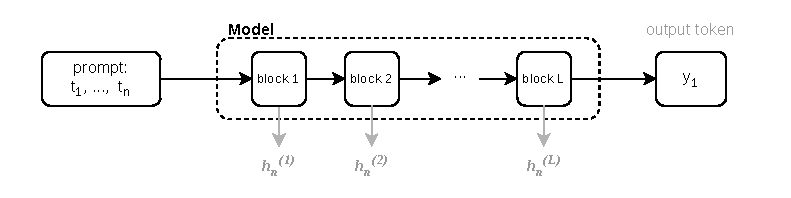
\includegraphics[width=0.9\textwidth]{images/hidden-states-ex.pdf}
	\caption[Hidden states across blocks]{The hidden states written at the last prompt token, $h^{(1)}_n, \dots, h^{(L)}_n$.}
	\label{fig:hidden-states}
\end{figure}

The set of these vectors is the representation that the model forms of the input while it processes it. At a fixed position, the vectors at increasing $\ell$ are successive states of the same representation, since each block reads the value produced by the previous one and writes an updated value into it. The prediction is refined block by block as a result \cite{gevaTransformerFeedForwardLayers2021, belroseElicitingLatentPredictions2025}. The content of these states depends on the layer. Ethayarajh measured how much the representation of a word varies with the context it appears in, on ELMo, BERT and GPT-2, and reported that the higher the layer, the more context-specific the representation is \cite{ethayarajhHowContextualAre2019}. After correcting for a property of these representations called anisotropy (Section~\ref{subsec:anisotropy}), Ethayarajh computed the first principal component of a word's representations across its contexts, a single fixed vector, and measured how much of the variation in those representations it explained. In every layer of the three models, on average, that vector explained less than 5\% of the variance in the word's representations across contexts. A word therefore has no small set of fixed senses that the model picks from: its representation differs in almost every context \cite{ethayarajhHowContextualAre2019}.

The last hidden state, $h^{(L)}_n$, is the vector to which the unembedding of Section~\ref{subsec:unembedding} is applied.

\subsection{Probing as a method}
\label{subsec:probing-method}

Reading a property off the hidden states is defined as \emph{probing}. A \emph{probe} is a classifier trained to predict a property of interest from the representations of a frozen model, and trained independently of the model itself \cite{alainUnderstandingIntermediateLayers2018a}. The representations are the input of the classifier and the property is its label, so the accuracy of the probe measures the degree to which the property is recoverable from the representation it is fitted on \cite{alainUnderstandingIntermediateLayers2018a}. Probing classifiers have become one of the main methods for analyzing neural models of natural language processing, and their methodological limitations have been reviewed critically \cite{belinkovProbingClassifiersPromises2021a}.

A probing result is limited both by what a high accuracy can establish and by the probe itself. A high accuracy establishes that a property is decodable from a representation. It does not establish that the model uses the property to produce its output \cite{belinkovProbingClassifiersPromises2021a}. Orgad et al. found that a model can encode the correct answer and consistently generate an incorrect one; this is the empirical form of the same distinction, since the property is present in the representation while the output does not reflect it \cite{orgadLLMsKnowMore2025}. The probe itself is a further limitation. A classifier with enough capacity can memorize the labels of the training data, achieving high accuracy even if the representation carries little of the property. In that case, the accuracy reflects the probe's own capacity, not the representation. A control baseline, a probe trained on the same task with the labels replaced by a version that carries no real signal, such as randomly shuffled labels, is therefore required: if the control also reaches high accuracy, the fitted probe's accuracy reflects its capacity to memorize rather than any property of the representation \cite{belinkovProbingClassifiersPromises2021a}.

A probe is commonly restricted to a linear classifier, because this matches how a property is expected to be encoded: not by one coordinate of the representation, but by its projection onto one fixed direction in the representation space, which is exactly what a linear classifier reads. Marks and Tegmark found that the truth or falsehood of a factual statement is linearly represented at sufficient model scale, and that shifting a representation along the identified direction changes the output of the model accordingly \cite{marksGeometryTruthEmergent2024}. Wu et al. reported the same form for the tool a model is about to call, which is carried by one direction per pair of tools and can be used to switch the selected tool \cite{wuToolCallingLinearly2026}. A linear probe's accuracy therefore measures whether the property is available as such a projection. Restricting the probe to a linear classifier also bounds its capacity, so the same kind of control baseline is needed to separate what the representation carries from what the probe learns from the labels \cite{belinkovProbingClassifiersPromises2021a}. With this control baseline in place, a high probe accuracy shows only that the property is decodable from the representation. It does not show that the model relies on this property when it produces its output.

\subsection{Anisotropy}
\label{subsec:anisotropy}

All representations of a given layer have high cosine similarity to each other, regardless of the word each one represents. This tendency is called \emph{anisotropy}: representations concentrate in a narrow region of the space instead of spreading in every direction \cite{ethayarajhHowContextualAre2019}. Anisotropy inflates the similarity between any two representations. For this reason, the measurement described in Section~\ref{subsec:hidden-states} is corrected before it measures how word-specific a representation is: Ethayarajh subtracted a baseline, the average similarity between representations of randomly sampled words at the same layer \cite{ethayarajhHowContextualAre2019}.

LatentGate, a hidden-state router discussed in Section~\ref{subsec:latentgate}, identifies anisotropy as a mechanism behind the failure of its embedding baselines, and corrects it with PCA-whitening before training its probe \cite{ratnakarLatentGateLowLatencySemantic2026}. Whether this correction helps a probe is debated. Forooghi et al. found the opposite pattern for classification tasks in large language models: whitening consistently degraded classification accuracy, across 8 models and 7 datasets \cite{forooghiWhiteningNotRecommended2024}.

\subsection{Choosing a Position to Probe}
\label{subsec:last-token}

Because attention in a decoder-only model is masked, the hidden state at position $i$ is computed from the first $i$ tokens only. Probing therefore requires a choice of which position to read the hidden state from, since different positions carry different information.

The last token of the prompt (Section~\ref{sec:terminology}) is the only position whose representation is computed with access to the entire prompt, and it is also the position from which the first generated token is predicted. Any information the model uses to select the first generated token has to be present in the hidden state at the last prompt token. As a result, the hidden state at the last prompt token carries the information behind the decision the model is about to state, before it produces any output token. A hidden state read at an earlier position instead carries only a partial representation of the prompt.

Healy et al. compared ten ways of extracting hidden states from a query, including reading the last token alone, and various pooling of all the token hidden states, and reported that detection accuracy varies with the choice, from 73.9\% to 74.6\% on their tool-call hallucination task \cite{healyInternalRepresentationsIndicators2026}. The probe position therefore influences the accuracy of the probe and should be evaluated for each task.

\subsection{Layer depth as an axis}
\label{subsec:layer-depth}

The layer index $\ell$ marks the depth at which a hidden state is read. Depth is an axis along which the content of the representation changes, and different layers can carry different amounts of information about a given property. Alain and Bengio introduced the practice of training an independent linear classifier on each layer of a frozen network. They used it to measure how suitable each layer's features are for a classification task, and reported on image classifiers that linear separability increases monotonically with depth \cite{alainUnderstandingIntermediateLayers2018a}. For language models the reported pattern is not monotonic: Azaria and Mitchell found that the accuracy of a truthfulness classifier depends on which layer supplies the activations, rather than being highest at the last one \cite{azariaInternalStateLLM2023}. Geva et al. and Belrose et al. gave a consistent account of why the layer index is informative: the representation is refined progressively, so its content differs between lower and upper blocks \cite{gevaTransformerFeedForwardLayers2021, belroseElicitingLatentPredictions2025}.

The number of blocks is not comparable across models: two models with similar parameter counts can differ in depth. Comparing layers across models therefore requires the depth index to be normalized by the total number of blocks rather than used directly.

\subsection{What the evidence supports}
\label{subsec:readability}

The claim that the intermediate values are informative rests on empirical results, not on an assumption. Belrose et al. showed that a probe trained on a single Transformer block decodes that block's hidden state into a usable prediction, and that the resulting trajectory of latent predictions can be used to detect malicious inputs with high accuracy \cite{belroseElicitingLatentPredictions2025}. Azaria and Mitchell trained a classifier on the hidden layer activations of a model as it reads or generates a statement, and obtained between 71\% and 83\% accuracy in labeling statements as true or false, depending on the base model \cite{azariaInternalStateLLM2023}. Orgad et al. reported that information of this kind is concentrated in specific tokens rather than spread uniformly across the sequence, and that exploiting this concentration improves error detection \cite{orgadLLMsKnowMore2025}. Wu et al. reported that which tool a model is going to call is encoded as a direction in activation space, and that this direction is readable before the call is generated \cite{wuToolCallingLinearly2026}. These results span distinct properties, factual truth, malicious intent, and tool selection, so decodability from the hidden state is not confined to one narrow signal.

These results hold under limits. Section~\ref{subsec:anisotropy} described a tendency of hidden states to already point in similar directions, corrected for before measuring how word-specific a representation is. Anisotropy means that two hidden states can have high cosine similarity for reasons unrelated to the property of interest, which constrains any method that compares hidden states directly. The constraint applies to methods that decide by similarity between representations, such as nearest-neighbour assignment or matching against a class centroid. It does not apply to a probe of the kind defined in Section~\ref{subsec:probing-method}, which is fitted on labelled examples and reads a direction in the space rather than a distance between two points. Orgad et al. further found that detectors trained on internal states fail to generalize across datasets \cite{orgadLLMsKnowMore2025}.

The results support a limited statement: a property is sometimes recoverable from the internal state of a model that does not state it, and whether it is recoverable in a given setting has to be measured rather than assumed.

